\chapter{Appendix}
\label{ch:appendix}

\section{Predictions on the Complete Test Partition}
\label{sec:appendix-gallery}

Figures~\ref{fig:gallery1} to \ref{fig:gallery3} show the output of the pooled v1+v2 model on
every one of the 48 held-out test images, so that the aggregate figures of
Chapter~\ref{ch:results} can be checked against the individual cases they summarise. The
confidence threshold is the value selected on the validation split, $t^{*} = 0.25$; nothing is
tuned to the images shown. Plaque-positive images are given first, ordered by file number, the
plaque-free images after them.

Two patterns are visible across the sheets. Where the model agrees with the annotation it tends to
agree closely, and the residual disagreement is usually one of extent rather than location: the
predicted region follows the same lesion but stops short of the annotated boundary or continues
past it. Where it fails on a plaque-free image, the predicted region is a thin ribbon running
along the vessel wall rather than a focal protrusion --- the failure mode discussed in
Section~\ref{sec:discussion-shared-errors}.

\begin{figure}[H]
\centering
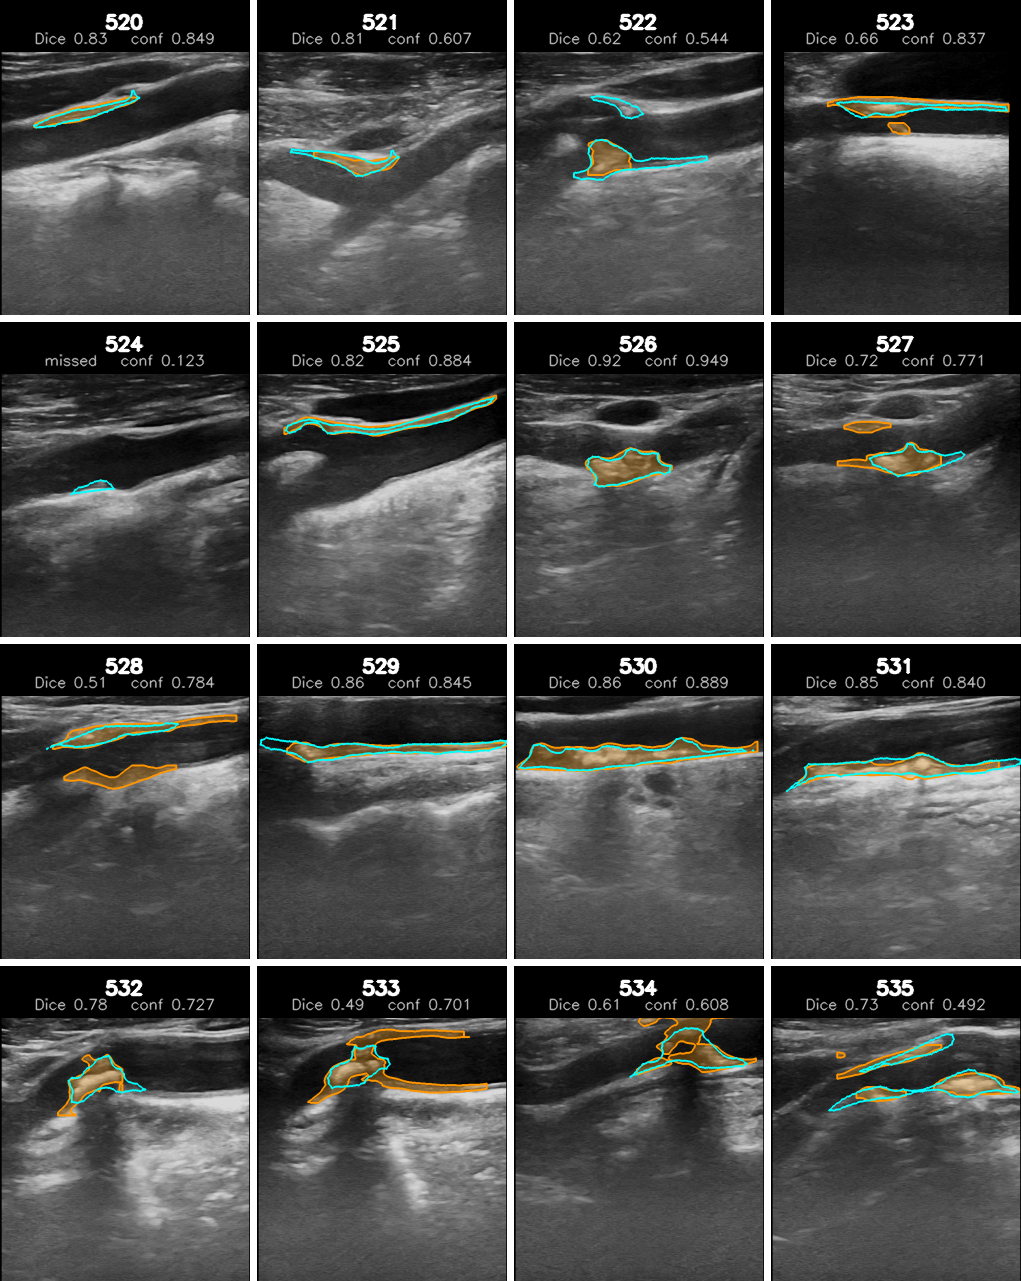
\includegraphics[width=\textwidth]{figures/appendix_gallery_1.png}
\caption[Test-set predictions, part 1]{Pooled v1+v2 predictions on test images 520--535, all
plaque-positive. The annotation is outlined in cyan, the prediction in orange with a light fill.
Each panel gives the Dice coefficient of the prediction against the annotation and the confidence
of the highest-scoring instance; ``missed'' marks an image in which no instance reached
$t^{*} = 0.25$.}
\label{fig:gallery1}
\end{figure}

\begin{figure}[H]
\centering
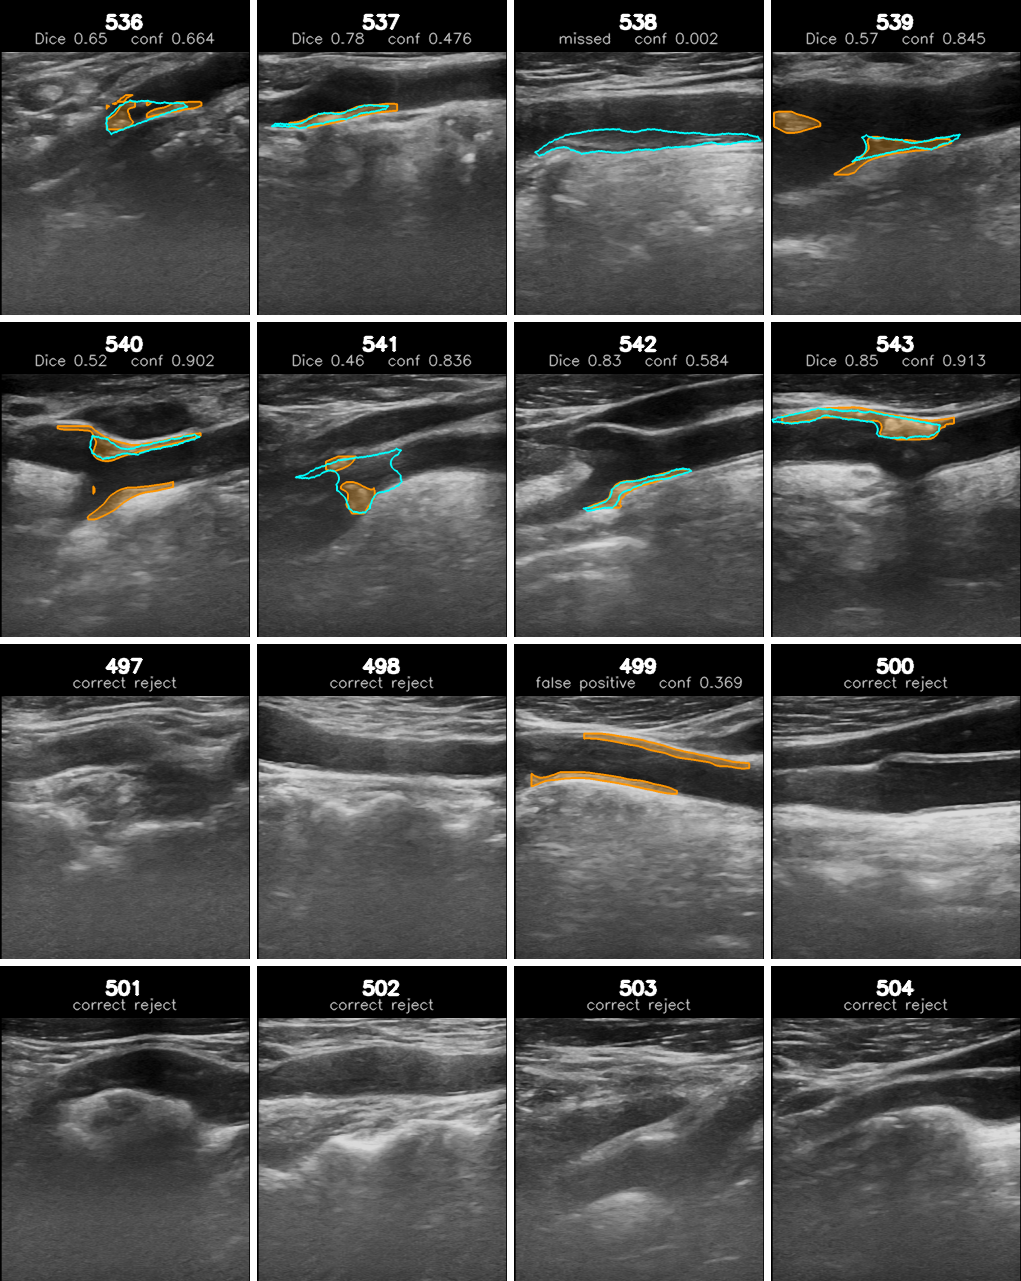
\includegraphics[width=\textwidth]{figures/appendix_gallery_2.png}
\caption[Test-set predictions, part 2]{Continuation of Figure~\ref{fig:gallery1}: the remaining
plaque-positive test images, followed by the first plaque-free ones. Colours and annotations as
in Figure~\ref{fig:gallery1}.}
\label{fig:gallery2}
\end{figure}

\begin{figure}[H]
\centering
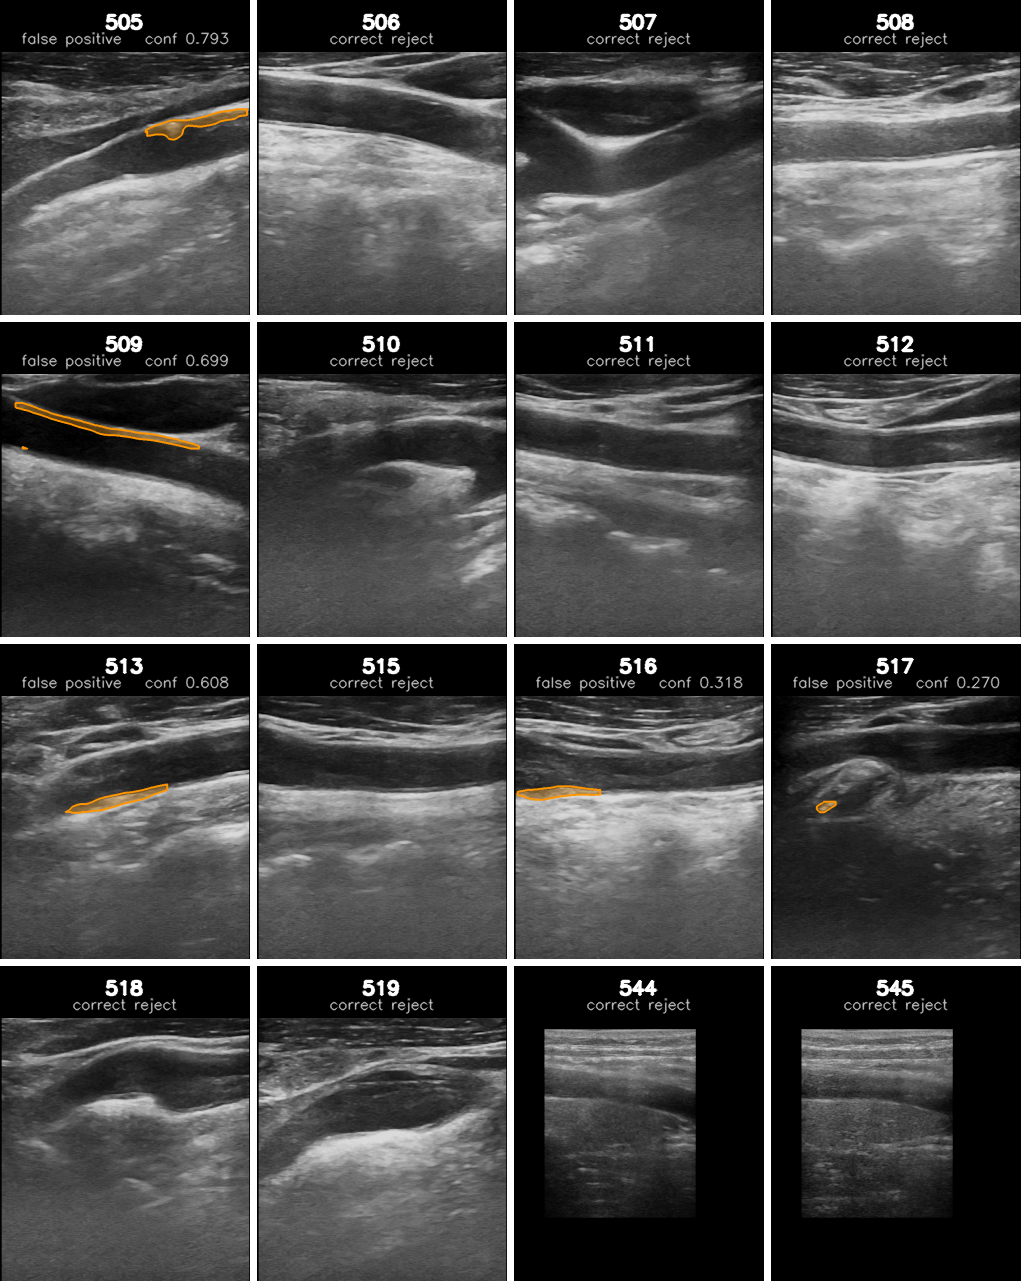
\includegraphics[width=\textwidth]{figures/appendix_gallery_3.png}
\caption[Test-set predictions, part 3]{The plaque-free test images. ``Correct reject'' marks an
image in which no instance reached the threshold; where one did, the panel is labelled as a false
positive and the predicted region is shown. The two images in the lower right were acquired with
the second device and differ visibly in field of view and gain.}
\label{fig:gallery3}
\end{figure}

\section{Per-Image Test Results}
\label{sec:appendix-per-image}

\begin{longtable}{lcccccccc}
\caption[Per-image test results]{Per-image results on the 48 held-out test images at the
operating points selected on the validation split. ``GT'' marks whether a plaque is annotated;
$\dagger$ marks the four images that also occur in the development partition. Check marks give
the image-level decision of seg\_v1, seg\_v2 and their union. ``Dice'' is the overlap achieved by
the union at its threshold, ``best'' the overlap of the best predicted instance irrespective of
its score, and ``conf'' the confidence that instance carries. Plaque-positive images are listed first, in the same order as Figures~\ref{fig:gallery1} to \ref{fig:gallery3}.}
\label{tab:per-image}\\
\hline
Image & GT & v1 & v2 & v1+v2 & Dice & best & conf \\
\hline
\endfirsthead
\hline
Image & GT & v1 & v2 & v1+v2 & Dice & best & conf \\
\hline
\endhead
\hline
\endfoot
520 & +$\dagger$ & \checkmark & \checkmark & \checkmark & 0.83 & 0.86 & 0.707 \\
521 & + & \checkmark & $\times$ & \checkmark & 0.81 & 0.81 & 0.607 \\
522 & + & \checkmark & \checkmark & \checkmark & 0.62 & 0.78 & 0.006 \\
523 & + & \checkmark & \checkmark & \checkmark & 0.66 & 0.77 & 0.012 \\
524 & + & $\times$ & $\times$ & $\times$ & 0.00 & 0.79 & 0.013 \\
525 & +$\dagger$ & \checkmark & \checkmark & \checkmark & 0.82 & 0.84 & 0.826 \\
526 & +$\dagger$ & \checkmark & \checkmark & \checkmark & 0.92 & 0.94 & 0.938 \\
527 & + & \checkmark & \checkmark & \checkmark & 0.72 & 0.90 & 0.003 \\
528 & + & \checkmark & \checkmark & \checkmark & 0.51 & 0.81 & 0.002 \\
529 & + & \checkmark & \checkmark & \checkmark & 0.86 & 0.85 & 0.053 \\
530 & +$\dagger$ & \checkmark & \checkmark & \checkmark & 0.86 & 0.91 & 0.889 \\
531 & + & \checkmark & \checkmark & \checkmark & 0.85 & 0.85 & 0.610 \\
532 & + & \checkmark & \checkmark & \checkmark & 0.78 & 0.80 & 0.012 \\
533 & + & \checkmark & \checkmark & \checkmark & 0.49 & 0.69 & 0.006 \\
534 & + & \checkmark & \checkmark & \checkmark & 0.61 & 0.61 & 0.529 \\
535 & + & \checkmark & \checkmark & \checkmark & 0.73 & 0.75 & 0.004 \\
536 & + & \checkmark & \checkmark & \checkmark & 0.65 & 0.72 & 0.001 \\
537 & + & \checkmark & $\times$ & \checkmark & 0.78 & 0.79 & 0.016 \\
538 & + & $\times$ & $\times$ & $\times$ & 0.00 & 0.82 & 0.002 \\
539 & + & \checkmark & \checkmark & \checkmark & 0.57 & 0.82 & 0.845 \\
540 & + & \checkmark & \checkmark & \checkmark & 0.52 & 0.76 & 0.104 \\
541 & + & \checkmark & \checkmark & \checkmark & 0.46 & 0.45 & 0.005 \\
542 & + & $\times$ & \checkmark & \checkmark & 0.83 & 0.83 & 0.584 \\
543 & + & \checkmark & \checkmark & \checkmark & 0.85 & 0.89 & 0.765 \\
497 & -- & \checkmark & \checkmark & \checkmark & -- & -- & -- \\
498 & -- & \checkmark & \checkmark & \checkmark & -- & -- & -- \\
499 & -- & $\times$ & \checkmark & $\times$ & -- & -- & -- \\
500 & -- & \checkmark & \checkmark & \checkmark & -- & -- & -- \\
501 & -- & \checkmark & \checkmark & \checkmark & -- & -- & -- \\
502 & -- & \checkmark & \checkmark & \checkmark & -- & -- & -- \\
503 & -- & \checkmark & \checkmark & \checkmark & -- & -- & -- \\
504 & -- & \checkmark & \checkmark & \checkmark & -- & -- & -- \\
505 & -- & $\times$ & $\times$ & $\times$ & -- & -- & -- \\
506 & -- & \checkmark & \checkmark & \checkmark & -- & -- & -- \\
507 & -- & \checkmark & \checkmark & \checkmark & -- & -- & -- \\
508 & -- & \checkmark & \checkmark & \checkmark & -- & -- & -- \\
509 & -- & $\times$ & $\times$ & $\times$ & -- & -- & -- \\
510 & -- & \checkmark & \checkmark & \checkmark & -- & -- & -- \\
511 & -- & \checkmark & \checkmark & \checkmark & -- & -- & -- \\
512 & -- & \checkmark & \checkmark & \checkmark & -- & -- & -- \\
513 & -- & $\times$ & $\times$ & $\times$ & -- & -- & -- \\
515 & -- & \checkmark & \checkmark & \checkmark & -- & -- & -- \\
516 & -- & $\times$ & $\times$ & $\times$ & -- & -- & -- \\
517 & -- & $\times$ & $\times$ & $\times$ & -- & -- & -- \\
518 & -- & \checkmark & \checkmark & \checkmark & -- & -- & -- \\
519 & -- & \checkmark & \checkmark & \checkmark & -- & -- & -- \\
544 & -- & \checkmark & \checkmark & \checkmark & -- & -- & -- \\
545 & -- & \checkmark & \checkmark & \checkmark & -- & -- & -- \\
\end{longtable}


\section{Instance-Level Performance of the Fine-Tuned Models}
\label{sec:appendix-training}

Chapter~\ref{ch:results} compares the fine-tuned models at the image level, which is the quantity
the downstream analyses consume. Figure~\ref{fig:appendix-pr} gives the complementary view at the
instance level, where each predicted plaque is matched against the annotation individually.

The four curves lie close together over the whole range, which is the same conclusion the
image-level evaluation reaches by a different route: the configurations differ in how they
distribute their errors rather than in how many they make. Two features are worth noting. None of
the models exceeds a recall of about 0.86 even at the lowest confidence, so a minority of
annotated instances is never produced at all. And precision falls below 0.5 well before that
point, so the instances added at low confidence are predominantly spurious --- which is why the
confidence threshold matters as much as it does, and why the ranking analysis of
Section~\ref{subsec:results-calibration} concerns the ordering rather than the masks.

\begin{figure}[H]
\centering
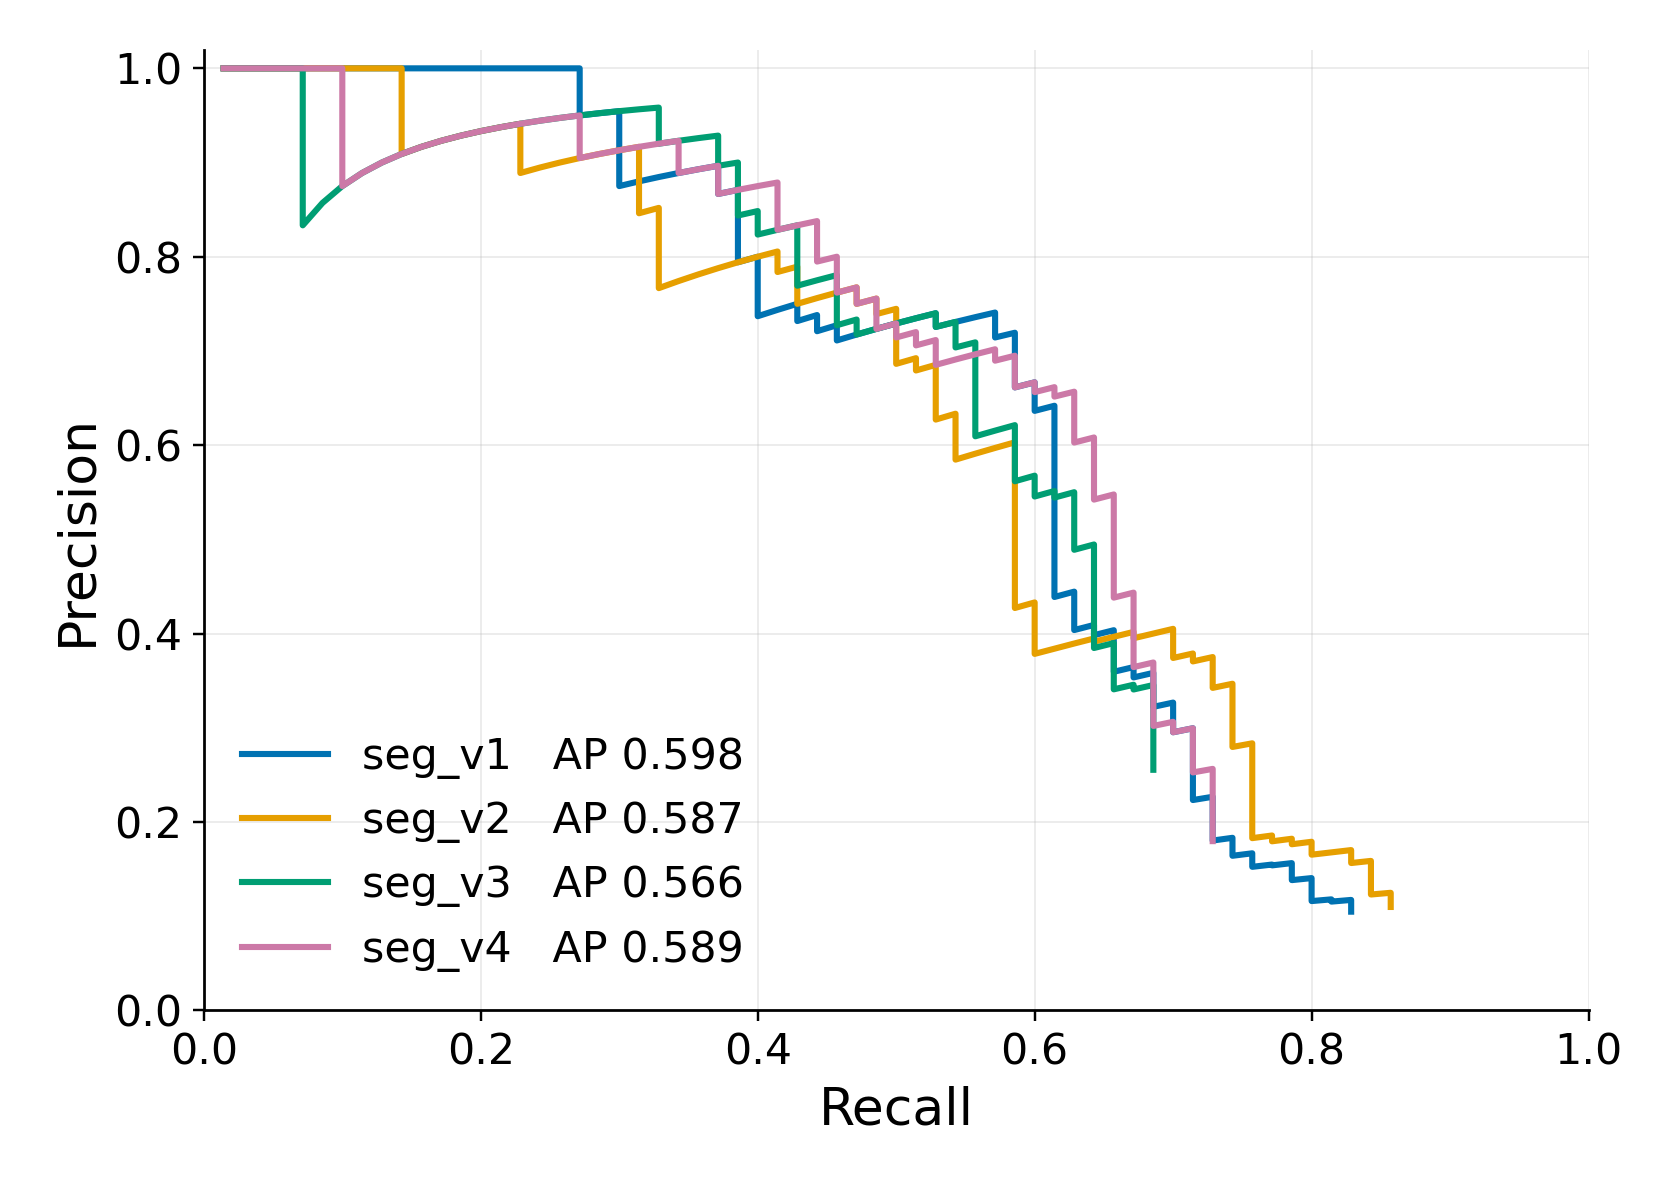
\includegraphics[width=0.86\textwidth]{figures/pr_curves.png}
\caption[Instance-level precision-recall curves]{Mask precision-recall curves of the four
fine-tuned configurations on the validation split. A predicted instance counts as a true positive
if its mask intersection over union with an as yet unmatched annotated instance reaches 0.5;
instances are matched in descending order of confidence, so each annotation is claimed at most
once. The legend gives the average precision, the area under the interpolated curve. The
evaluation covers 70 annotated instances across the 73 validation images.}
\label{fig:appendix-pr}
\end{figure}

